\RequirePackage[2020-02-02]{latexrelease}


% Template for seminar reports
% Computer Vision Group, Visual Computing Institute, RWTH Aachen University
\documentclass[twoside,a4paper,article]{combine}
\usepackage[utf8]{inputenc}
\usepackage{a4}
\usepackage{fancyhdr}   
%\usepackage{german}    % Uncomment this iff you're writing the report in German
\usepackage{makeidx}
\usepackage{color}
\usepackage{t1enc}		% German letters in the "\hyphenation" - command
\usepackage{latexsym}	% math symbols
\usepackage{amssymb}    % AMS symbol fonts for LaTeX.
\usepackage{graphicx}
\usepackage{pslatex}
\usepackage{ifthen}
\usepackage{booktabs}
\usepackage[T1]{fontenc}
\usepackage{pslatex}
\usepackage{psfrag}
\usepackage{subfigure}
\usepackage{url}
\usepackage{datetime}
\usepackage{xspace}
\usepackage{newtxmath}

\usepackage{float}
\usepackage{subcaption}

\newdateformat{monthyeardate}{\monthname[\THEMONTH] \THEYEAR}

% Do not change these sizes and do not add superfluous 
% pagebreaks to increase the page count.
\setlength{\oddsidemargin}{3.6pt}
\setlength{\evensidemargin}{22.6pt}
\setlength{\textwidth}{426.8pt}
\setlength{\textheight}{654.4pt}
\setlength{\headsep}{18pt}
\setlength{\headheight}{15pt}
\setlength{\topmargin}{-41.7pt}
\setlength{\topskip}{10pt}
\setlength{\footskip}{42pt}
\setlength{\parindent}{0pt}

\makeatletter
\DeclareRobustCommand\onedot{\futurelet\@let@token\@onedot}
\def\@onedot{\ifx\@let@token.\else.\null\fi\xspace}
\def\eg{\emph{e.g}\onedot} \def\Eg{\emph{E.g}\onedot}
\def\ie{\emph{i.e}\onedot} \def\Ie{\emph{I.e}\onedot}
\def\cf{\emph{c.f}\onedot} \def\Cf{\emph{C.f}\onedot}
\def\etc{\emph{etc}\onedot} \def\vs{\emph{vs}\onedot}
\def\wrt{w.r.t\onedot} \def\dof{d.o.f\onedot}
\def\etal{\emph{et al}\onedot}
\makeatother

% =========================================================================
\graphicspath{{pictures/}}
\setcounter{secnumdepth}{3}
\setcounter{tocdepth}{3}

% =========================================================================
\begin{document}
% Template for seminar reports
% Seminar Current Topics in Computer Vision and Machine Learning


\begin{titlepage}
    \begin{center}
    \ 
    \vspace{3.5cm}
    
    \textsf{
    RWTH Aachen University \\
    Faculty of Mathematics, Computer Science and Natural Sciences\\
    Chair of Computer Science 13 (Computer Vision) \\
    Prof. Dr. Bastian Leibe
    }
    
    \rule{\linewidth}{1pt}
    
    \vspace{1.75cm}
    \LARGE
    \textbf{Seminar Report}
    
    \vspace{1.7cm}
    \huge
    Linear and Nonlinear Filters
    
    \vspace{3.0cm}
    \Large
    Alexander Skretting\\
    \large
    Matriculation Number: 445457

    \vspace{1.0cm}
    \Large
    Jose Rigel Soeryo Soebandoro\\
    \large
    Matriculation Number: 444345
    
    \vspace{0.5cm}
    \monthyeardate\today
    
    \vspace{1.05cm}
    \rule{\linewidth}{1pt}
    
    \vspace{0.5cm}
    \textsf{\textbf{
    \normalsize
    \begin{tabular}{ll}
    Advisor:  & George Lydakis\\
    \end{tabular}
    }}
    \end{center}
\end{titlepage}



\begin{abstract}
% +++++++++++++++++++++++++
% Insert your Abstract here (one paragraph summary)
% +++++++++++++++++++++++++
\end{abstract}

\tableofcontents
\newpage
% =========================================================================

\section{Introduction}
\section{Linear Filters}
With \textbf{Linear Filtering}, or specifically linear spatial filtering, the function which is used to pass the image through
must be linear and shift invariant.\smallskip

A common formula for linear filtering is the \emph{Correlation Filtering}. \cite{BovikActon09}
\[
    g(i,j) = \sum_{l \in \mathscr{M}}\sum_{k \in \mathscr{N}}{f(i+k, j+l) \cdot h(k, l)}
\]
or commonly notated as $g = f \otimes h$.\smallskip

The desired output pixel $g(i, j)$, where $i$ and $j$ specify the
coordinates of it, is based on a $M \times N$ sized neighborhood, 
meaning not only does one pixel define an output pixel, but also a specified number
of its neighbors. The influence of each pixel in the neighborhood is defined by the filter coefficient $h(k, l)$,
also called its \emph{kernel} or \emph{mask}. \cite{Szeliski_2022}\smallskip

$$
\underbrace{
    \begin{bmatrix}
        128 & 34 & 123\\
        68 & 54 & 73 \\
        100 & 95 & 17
    \end{bmatrix}}_{\text{input neighborhood}}
\otimes
\underbrace{
    \begin{bmatrix}
        0.1 & 0.1 & 0.1\\
        0.1 & 0.2 & 0.1\\
        0.1 & 0.1 & 0.1
    \end{bmatrix}}_{\text{kernel}}
= 75
$$

As the above example with a $3 \times 3$ kernel, a total of 9 pixels is needed to calculate a single output pixel.\smallskip

Another common variant on the formula is having the signs of the offsets reversed. 
\[
    g = f \ast h
\]
\[
    g(i,j) = \sum_{l \in \mathscr{M}}\sum_{k \in \mathscr{N}}{f(i-k, j-l) \cdot h(k, l)}
\]
With this formula, $\ast$ is called the \emph{convolutional} operator, and the kernel $h$ is called the \emph{impulse response function}. 
An interesting note is that, when the kernel $h$ is convolved with an impulse signal $\delta$ (an image with 0 everywhere except the origin),
it reproduces the kernel itself $h \ast \delta = h$, whereas with correlational filtering, 
it produces the reflected signal (inverted signal in both dimensions).\cite{Szeliski_2022} In cases
where the kernel is symmetrical on both axis (e.g. box blur), the result of convolutional and correlational is the same.

\begin{minipage}{\textwidth}\begin{figure}[H]
    \centering
    \subfigure[correlation]{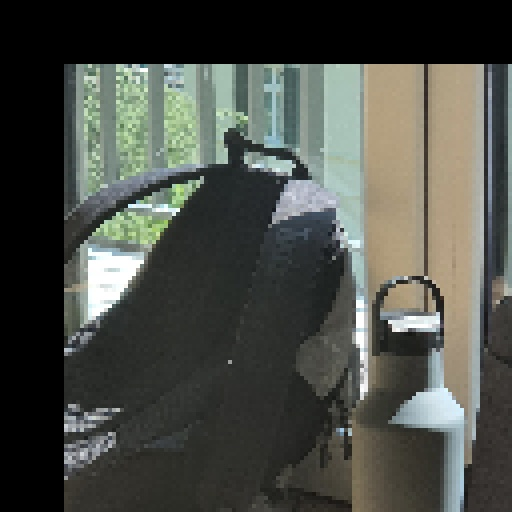
\includegraphics[width=0.19\textwidth]{img/correlation.jpg}}
    \subfigure[convolution]{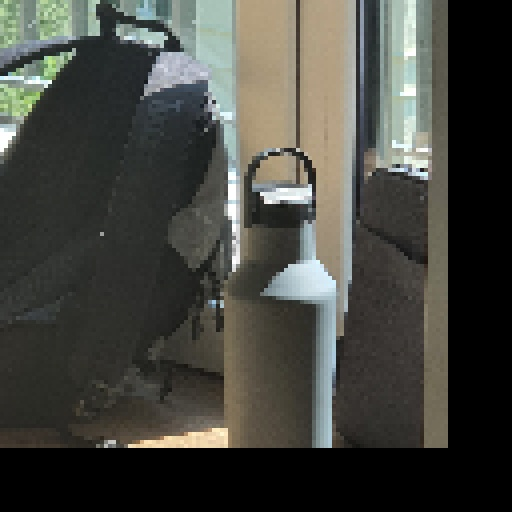
\includegraphics[width=0.19\textwidth]{img/convolved}}
    \caption{Difference between Correlation and Convolution Filtering by translating 32 pixels}
    \label{fig:correlation_convolution}
\end{figure}\end{minipage}\smallskip

An apparent problem from neighborhood filtering is that on the edges, the neighbors simply does not exist in one or two directions 
(e.g. a $1000\times1000$ image passed through a $3\times3$ kernel would produce a $998\times998$ image). 
There are a couple method to alleviate the calculation of the nonexistent neighbors.


\subsection{Padding (Border Effects)}

\begin{minipage}{\textwidth}\begin{figure}[H]
    \centering
    \subfigure[zero]{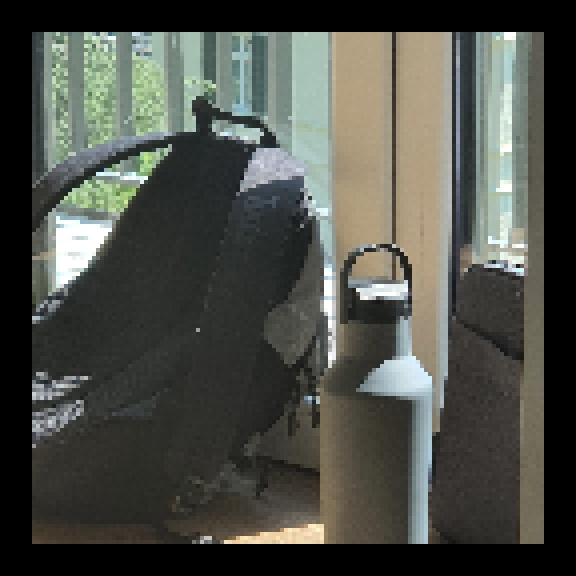
\includegraphics[width=0.19\textwidth]{img/border_constant}}
    \subfigure[wrap]{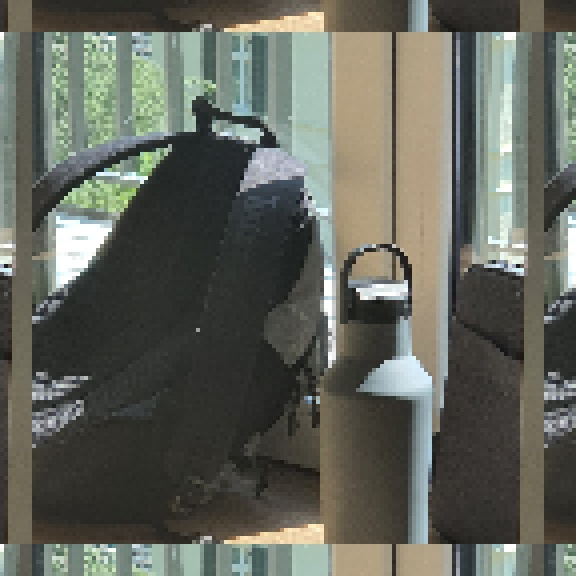
\includegraphics[width=0.19\textwidth]{img/border_wrap}}
    \subfigure[clamp]{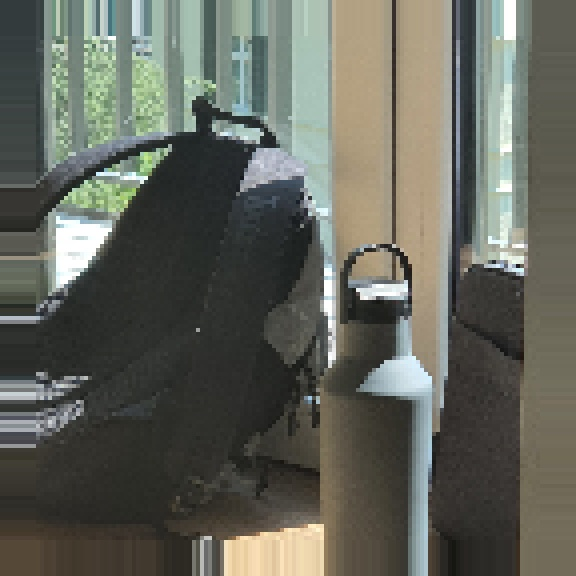
\includegraphics[width=0.19\textwidth]{img/border_clamp}}
    \subfigure[mirror]{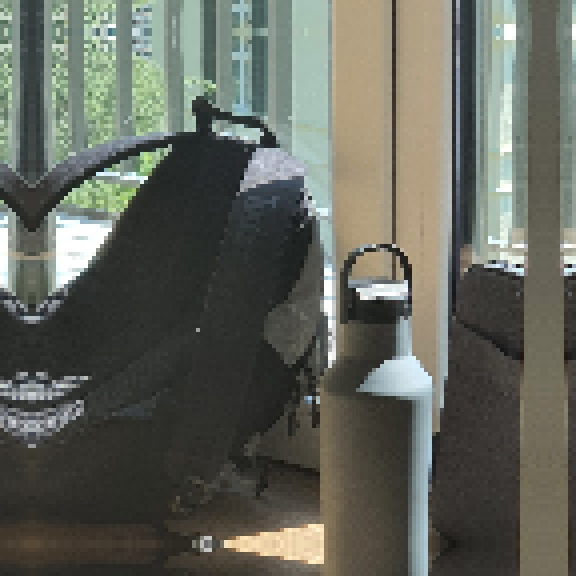
\includegraphics[width=0.19\textwidth]{img/border_reflect}}
    \subfigure[extend]{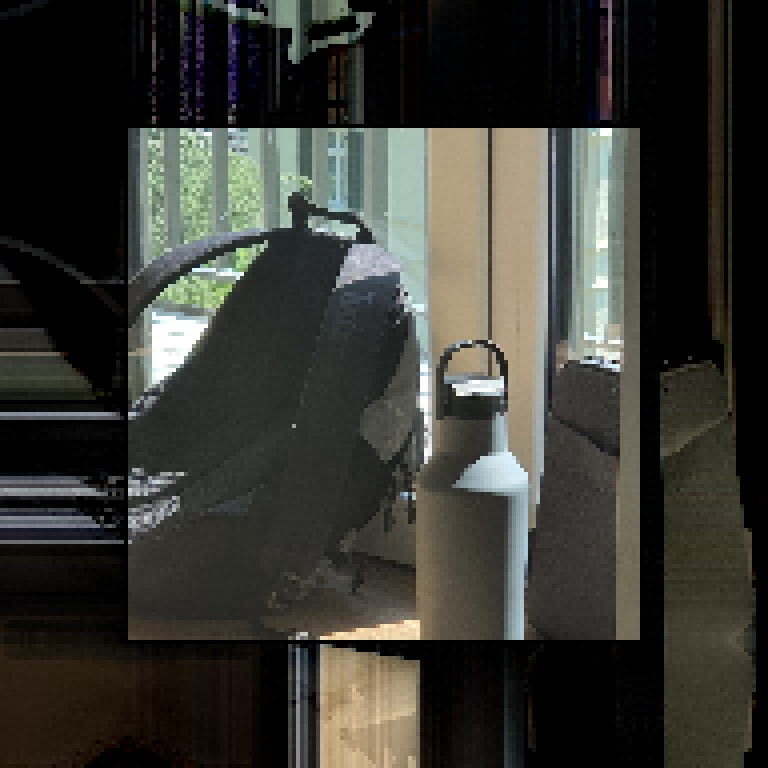
\includegraphics[width=0.19\textwidth]{img/border_extend.jpg}}
    \caption{Different types of border padding}
    \label{fig:padding_borders}
\end{figure}\end{minipage}
\begin{itemize}
    \item \textbf{Zero:} Set all pixels outside the region to zero.
    \item \textbf{Constant:} This is similar to Zero, but instead a specific color is chosen to replace the out of bound pixels.
    \item \textbf{Clamp:} The edge pixels are repeated indefinitely.
    \item \textbf{(Cyclic) Wrap (Repeat or Tile):} The entire image is repeated similar to tiling it infinitely.
    \item \textbf{Mirror:} The image is mirrored accordingly on each of the edges.
    \item \textbf{Extend:} This is a combination of clamping and mirroring, where clamped image is subtracted with the mirrored image.
\end{itemize}

This of course not only affects the unseen pixels, but the effects can bleed into the pixels inside the frame.
\begin{minipage}{\textwidth}\begin{figure}[H]
    \centering
    \subfigure[zero]{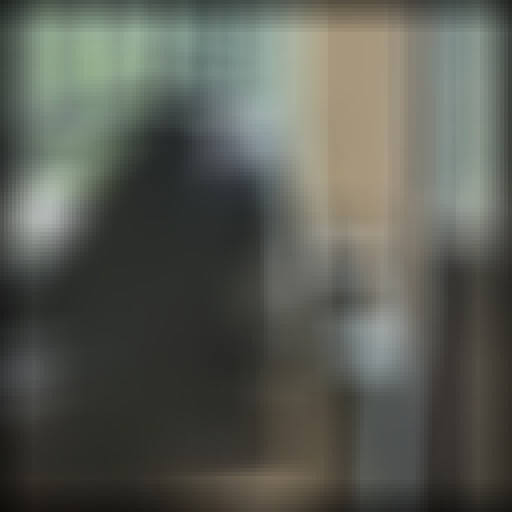
\includegraphics[width=0.19\textwidth]{img/boxBlur_constant}}
    \subfigure[wrap]{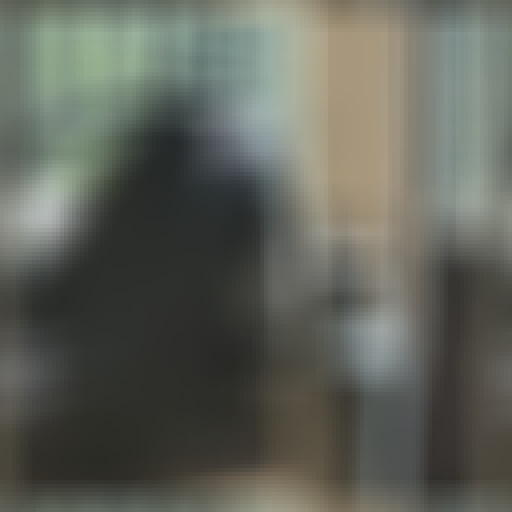
\includegraphics[width=0.19\textwidth]{img/boxBlur_wrap}}
    \subfigure[clamp]{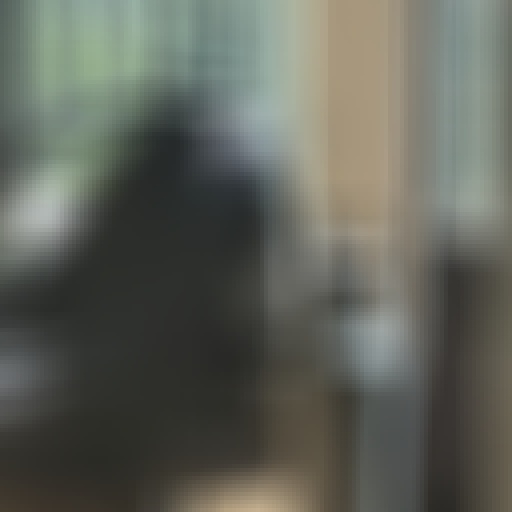
\includegraphics[width=0.19\textwidth]{img/boxBlur_clamp}}
    \subfigure[mirror]{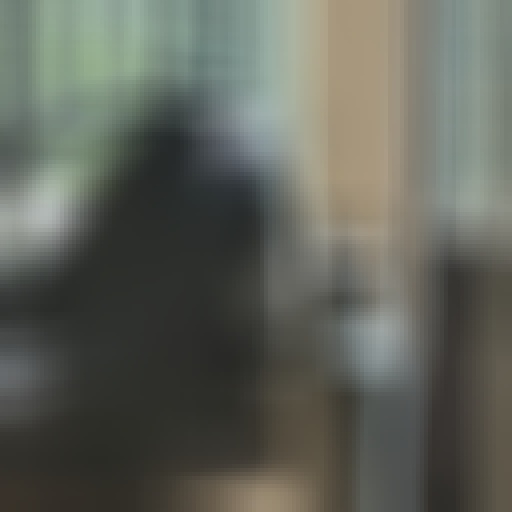
\includegraphics[width=0.19\textwidth]{img/boxBlur_reflect}}
    \subfigure[extend]{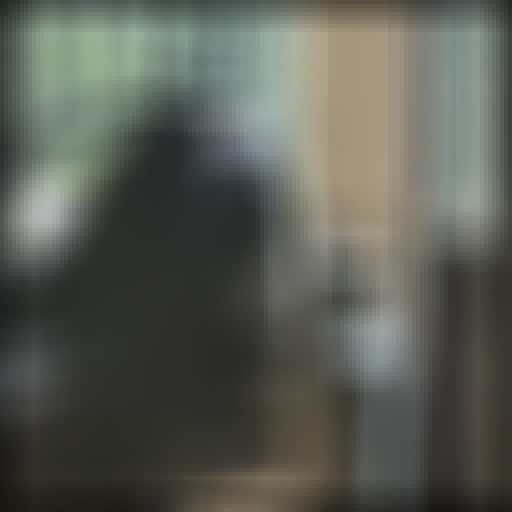
\includegraphics[width=0.19\textwidth]{img/boxBlur_extend.jpg}}
    \caption{Effects of different paddings with box blur}
    \label{fig:boxBlur_borders}
\end{figure}\end{minipage}\smallskip

There are other ways to handle the borders such as two-phase duplication,
which is similar to clamp but alternates between the last 2 pixels.
A change in the filter function per individual basis can also be implemented, but it might not be practical,
as large amounts of additional logic may be needed. \cite{BaileyAmbikumar18}

% =========================================================================
\bibliographystyle{alpha}
\bibliography{abbrev, Draft}
\end{document}
